% !TeX spellcheck = en_US
\chapter{Expansion of a semantic model for emotion-related descriptors}
\label{Chap:ANEW}
One of the fundamental properties of music is the ability to convey emotions\cite{Yang2012}. Consequently, the Music Information Retrieval has been greatly interested in representing and classifying music according to emotions for music recommendation and personalization \cite{Juslin:2001, Juslin2011, Lee2004, Yang2012}. Traditional meta-tags like artist or title are not informative on the content of a music piece and several studies \cite{Juslin:2001, Juslin2011, Lee2004, Yang2012} on music information needs and on user behaviors have proven, in fact, the interest of representing and classifying music according to emotions.
It has been proven that listeners enjoy looking for and discovering music using mood-based queries, which represents 33\% of music queries according to \cite{Lee2004}. This is an important reason that urged psychologist and musicologist to investigate different paradigms for the representation and modeling of emotion related descriptors \cite{Juslin:2001, Juslin2011, Lee2004}. 

In Section \ref{sec:HLFs:VA} we presented the Valence-Arousal (VA) model, which is one of the most widely used semantic model for the representation of emotional-related descriptors and content. The Valence is linked to the degree of pleasantness, while the Arousal represents the degree of excitement, or activation. A third dimension related to \textit{Dominance} (D) was later proposed to express the degree of control and to possibly distinguish different and overlapping moods \cite{Cowie2012, Scherer2004}, leading to the Valence, Arousal, Dominance (VAD) space. In Section \ref{sec:HLFs:VA} we also discussed about the \textit{Affective Norm for English Words} (ANEW) dataset \cite{Bradley1999}, which is composed of almost 2,500 emotional-related descriptors mapped in the VAD space. While the dataset has been a helpful resource for the MIR community, it was not specifically designed for music description, and it therefore presents some difficulty on their use. As an example, it is not sure whether the metric of distance defined in the VA/VAD space can match the semantic similarity for the context of music description. Moreover, due to the clutter distribution of terms (see Figure \ref{fig:ANEW:ANEW}) it is difficult to conceptually organize them into a  hierarchy that is closer to how people describe music.

\begin{figure}[bt] 
	\centering 
	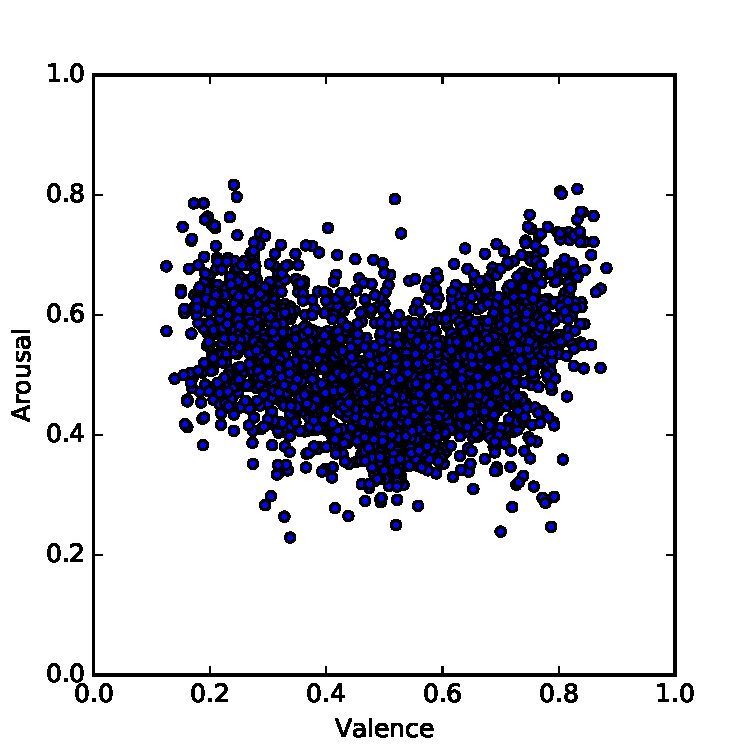
\includegraphics[width=0.9\columnwidth]{img/ANEW/ANEW.pdf}
	\caption{Distribution of the ANEW dataset in the VA space}
	\label{fig:ANEW:ANEW}
\end{figure}	

In this study, we investigate the production of a different emotional space, where the terms from ANEW dataset are better conceptually organized and bear more relevance for music description. This study only concerns a transformation of the semantic codomain and it does not involves the music signals. Such emotional space, however, would be highly helpful for the development of novel music mediators, by providing a reliable semantic model for dimensional descriptors. In this scenario, the domain and the codomain of the problem both lie in the semantic world, and we aim at finding a linking function that is able to shape the VA or VAD semantic model to the novel space.

We build the new emotional space by taking advantage of kernel expansion techniques applied to the VA and VAD space, in order to design higher-dimensional emotional spaces.  Although the kernel transformation has the effect to produce a more sparse distribution of terms, it is not clear if the  semantic distance between concepts is well represented by the metric in the new space. To solve this problem, we first aim to find a distance reflecting conceptual organization of terms by applying distance learning techniques \cite{xing2003distance, bar2003learning, goldberger2004neighbourhood} (as discussed in Section \ref{sec:ML:dist}). Given some constraints between terms, these methods search for a linear transformation of the space that is semantically relevant. That is, the ideal learned distance closely correlates with semantic differences given by users in a specific task for a subset of the ANEW terms. We generate the set of constraints using ``a priori'' information collected through a subjective test where participants were asked to specify the semantic similarity between pairs of terms in the context of music. We then perform Latent Semantic Analysis on emotion related annotations for a large set of music pieces. 

Under the hypothesis that the terms may be improved by this transformation, we validate the approach by grouping (i.e.,  clustering) the descriptors in the new high-dimensional space. In order to isolate the effect of distance learning from the use of apriori constraints, we use both unsupervised clustering techniques and semi-supervised clustering techniques. The latter make use of the same kind of constraints to retrieve the clusters with more relevance to the music semantics. We subsequently evaluate the resulting clusters with objective and subjective metrics. Tests show promising results given these new learned distance metrics and provide an insight into how a better configuration in the high-dimensional space can be achieved. 


 \begin{figure}[tb] 
 	\centering 
 	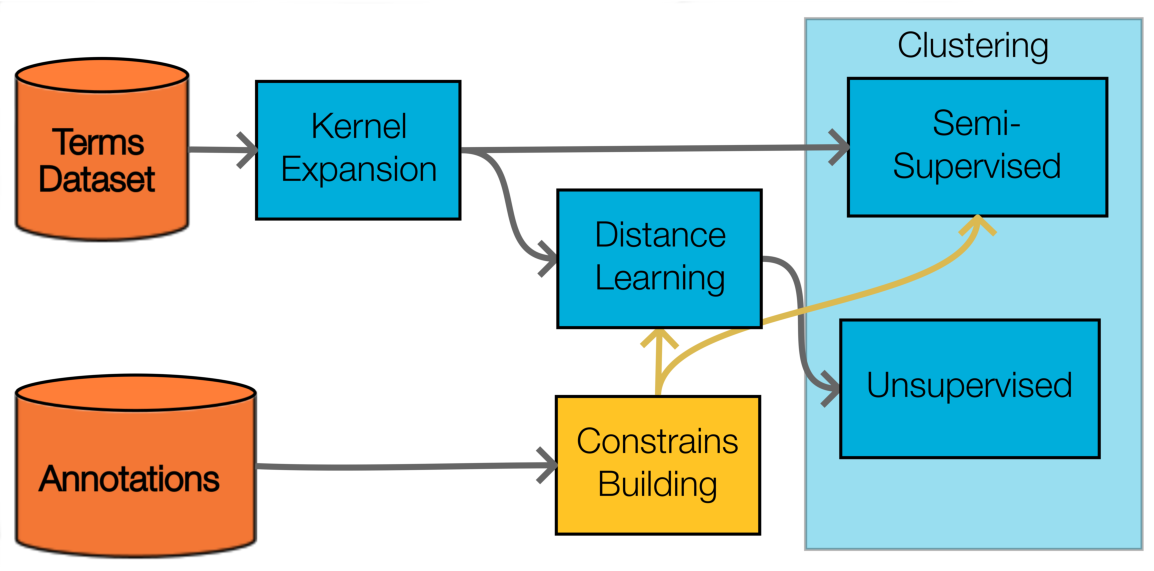
\includegraphics[width=0.95\columnwidth]{img/ANEW/scheme4.pdf}
 	\caption{Block diagram of the clustering approach}
 	\label{fig:ANEWblockdiag}
 \end{figure}	

Figure \ref{fig:ANEWblockdiag} shows the scheme of this work. We discuss the collection and generation of the annotated data and the building of the constraints to embed semantics about music in the learned distance metrics. We provide some quick details on the kernel expansion and distance learning techniques, since a more extensive dissertation was presented in Sections \ref{sec:ML:kernels} and \ref{sec:ML:dist}, respectively. We then present the clustering techniques and the numerical results on the resulting clusters. Finally, we draw some overall considerations on the work.


\begin{table}
\begin{center}
\bgroup
\def\arraystretch{1.5}
\begin{tabular}{ ||p{.12\columnwidth} |l |p{.13\columnwidth}  |p{.50\columnwidth}||}
% \hline
\hline
\hline
Type &  Symbol & Num Terms & Details \\
\hline
\hline
Terms Dataset  &$\mathcal{D}_{ANEW} $ %=\{\mathbf{w}_1, ..., \mathbf{w}_N\}$
& 2,476 & Mean in V, A, D dimensions\\
% \hline
\hline
Implicit Distance  &$\mathbf{M}_{ILM10K}$& 240, 450 & Tag compact representation from an LSA with $k=10,20,50,100$ components\\
\hline
Explicit Distance  & $\mathbf{M}_{HD} $ & 180 & Human annotation of semantic similarity between terms from ANEW\\
\hline
Explicit Clustering  & $\mathbf{M}_{HC} $ & 100 & Human clustering of a subset of ANEW\\
\hline
\hline
% \hline
\end{tabular}\quad
\egroup
\end{center}
\caption{Summary of the collected data}
\label{tab:ANEWdata}
\end{table}


\section{Collection of the dataset}\label{sec:ANEW:data}
In this section, we describe three datasets created to provide constraints for semi-supervised learning as well as to validate our approach. A summary of the collected data is provided in Table \ref{tab:ANEWdata}.

\subsection{Terms in the ANEW Dataset}
The terms in the ANEW dataset \cite{Bradley1999} is already annotated for the Valence, Arousal and Dominance dimensions with a value between 0 and 10 by Psychology class students. For each term, we consider the normalized average (between 0 and 1) of the annotations. We will refer to the ANEW dataset as
\begin{equation}
\mathcal{D}_{ANEW}=\{\mathbf{w}_1, ..., \mathbf{w}_T\}
\label{eq:ANEW:ANEW}
\end{equation} 
with $\mathbf{w}_i=\{\mu_V, \mu_A, \mu_D \}$ and $T=2476$. Specifically, we will refer to $\mathcal{D}_{ANEW}^{(AV)}$ and $\mathcal{D}_{ANEW}^{(VAD)}$ as the dataset with only Arousal and Valence dimensions considered and the dataset with also Dominance considered, respectively. 

\subsection{Implicit Distance Annotation}
\label{sec:ANEW:ILM}
In Section \ref{sec:HLFs:LSA} we explained how we can perform  Latent Semantic Analysis (LSA) on an annotated dataset in order to infer a dimensional semantic model, which include a metric of similarity among songs or terms. In this study, we compute a self-distance matrix among emotion related descriptors by performing LSA on a dataset composed of 10,199 tracks annotated with crowd sourced editorial and social tags, named I-Like-Musik dataset, or ILM10K \cite{Saari2015, Allik2016}.
The dataset is annotated with weights corresponding to the prevalence of each tag in each song description. 

From the tags in ILM10K, we first discard the tags that are not included in the ANEW dataset. We then filter the tags that are rarely used by thresholding the frequency with which the tag  was used in ILM10K. We empirically choose the two thresholds as $15$ and $5$ times, leading to a set of $T=240$ and $T=450$ terms respectively. The former vocabulary contains less terms, but it is more reliable since they have been used quite often, while the latter is richer but might carry a lower degree of information. 

Using the remaining tracks, we build a track-tag matrix, of which we compute a $k$-component approximation via LSA. We keep different numbers of components $k=10, 20, 50, 100$ to test different degrees of approximation, and we produce the set of matrices $\mathbf{D}_{ILM10K}^{(T,k)} \in \mathbb{R}^{T \times k} $. 
 
Given a generic approximated matrix $\mathbf{D}_{ILM10K}$ (i.e., neglecting the notation about $T$ and $k$ for the sake of clarity), we compute two self-distance matrices between tags, using the Euclidean distance between the correspondent rows, producing the matrix  $\mathbf{M}_{ILM10K}$, and between the normalized rows (i.e.  $\mathbf{\tilde{D}}_{ILM10K}$, producing the matrix $ \tilde{\mathbf{M}}_{ILM10K}$. The latter matrix can be seen as a kind of transformation of the self-distance matrix using the Cosine distance.

\subsection{Human Distance Annotation}
\label{sec:ANEW:HDA}
We conducted an online survey to collect information on how people think of and rate the actual semantic similarity among emotional-related descriptors in the music context. Each tester was asked to define the perceived mood similarity in the context of music between pairs of descriptors with a value between $0$ (not similar at all) and $1$ (very similar). In order to have an annotation similar to that collected in Section \ref{sec:ANEW:ILM}, we inverted the score so that $0$ becomes the value for maximum semantic similarity and vice versa.

504 people participated in the survey. In order to have only robust and reliable annotations, we kept only the terms that received at least 2 annotations leading to $T=180$. With the collected annotations, we compose the sparse matrix $ \mathbf{M}_{HD}$.

\subsection{Human Clustering Annotation}
\label{sec:ANEW:HCA}
Since we evaluate our approach by clustering the terms in the ANEW dataset in the original and new space, we also collected data on how people organize and group the emotional-related descriptors.

Therefore, we conducted a second online survey and asked annotators to group the set of top $100$ descriptors in the dataset. We did not provided a fixed number of clusters, nor any suggestion or guideline, in order to collect the most possible unbiased annotations. 

At first, the testers were presented with the list of $100$ descriptors and an empty list of clusters. Testers were able to create as many clusters as they felt to need for their organization. 

$15$ people participated in the survey, leading to the matrix $\mathbf{M}_{HC} $ with $T=100$ terms, where each entry $(i,j)$ indicates the number of people that grouped together the $i$-th and $j$-th terms. 

The number of testers that conducted the second study is sensibly lower with respect to the first survey in Section \ref{sec:ANEW:HDA}. This is due to the high cognitive load of the task and the impossibility to use partially-annotated information. However, the information provided by $\mathbf{M}_{HC}$ is actually rich enough for the scope of our work. Indeed, while the matrix $ \mathbf{M}_{HD}$ is a sparse matrix, i.e., some pairs of terms might have not received any annotation, the matrix $\mathbf{M}_{HC} $ is a full matrix. Whenever $\mathbf{M}_{(HC)}(i,j)=0$, we can infer that all the $15$ testers have annotated that the $i$-th and $j$-th terms are too semantically dissimilar to be grouped in the same cluster. 

\begin{figure}[bt] 
	\centering 
	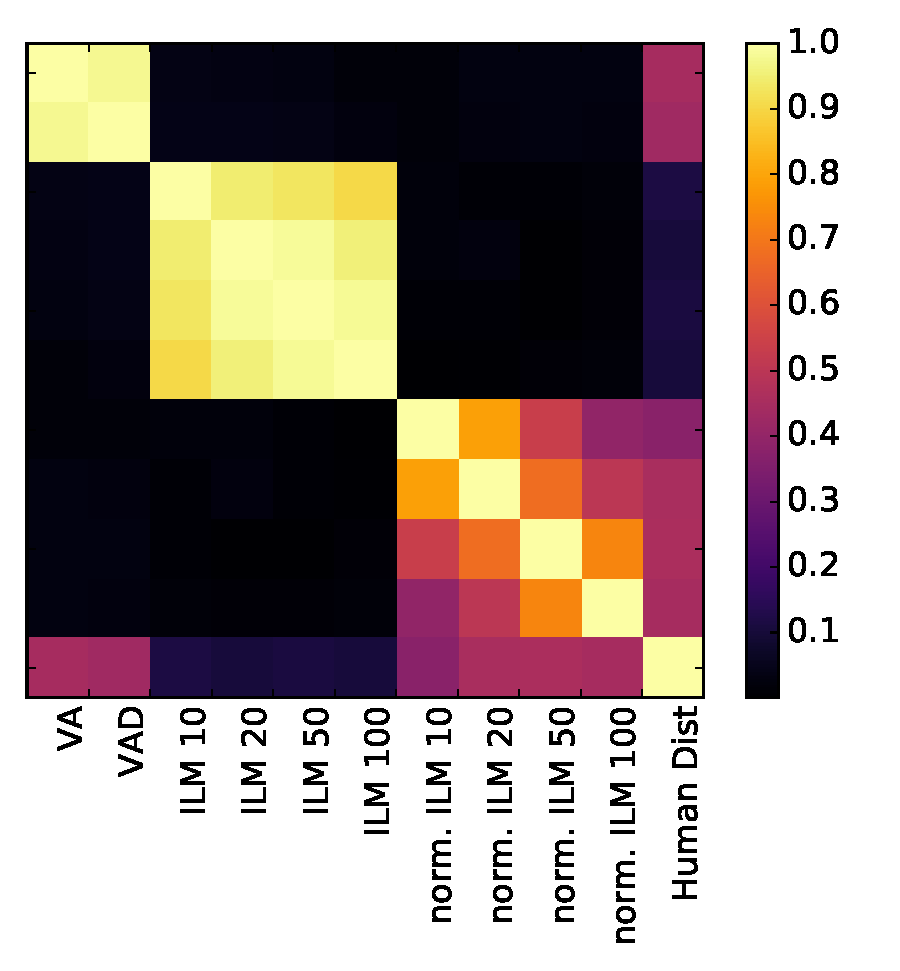
\includegraphics[width=0.80\columnwidth]{img/ANEW/pearson_dist_3.pdf}
	\caption{Absolute Pearson Correlation of the self-similarity matrices computed or collected from different sources of data.}
	\label{fig:ANEWdistData}
\end{figure}	

\subsection{Preliminar considerations on data}
In Figure \ref{fig:ANEWdistData} we show the absolute Pearson correlations between the self-distance matrices from different sources of data we collected. We can see that there is absolutely no correlation between the Euclidean distance defined in the VA or VAD space and the one that can be inferred from the LSA of the ILM10K dataset. Moreover, it exhibits a modest correlation also with the human distance annotation. This confirms the need of a new space for the ANEW dataset which is more similar to the music description.

\section{Learning the high-dimensional semantic space}
\label{sec:ANEW:moodtag}
We aim at producing a new space for the ANEW dataset by exploiting high-dimensional transformations of the VA or VAD space. In order to do this, we employ kernel expansions and distance learning techniques, as presented in Sections \ref{sec:ML:kernels} and \ref{sec:ML:dist}.

As far as the kernels are regarded, we employ the polynomial (degree 2 and 3) and RBF kernels described in \ref{sec:ML:kernels} in their explicit form. We also consider two non high-dimensional cases:
\begin{itemize}
\item we use the simple data in $\mathcal{D}_{ANEW}$ as-is, in order to take into consideration the non-expanded case and compare the new space with the traditional VA or VAD space;
\item we make use of the $L^2$ normalized data, by compose the dataset $\tilde{\mathcal{D}}_{ANEW}$ with the terms $\{\tilde{\mathbf{w}}_1,..., \tilde{\mathbf{w}}_T \}$, where each term is the $L^2$-normalized of the terms in $\mathcal{D}_{ANEW}$, i.e., 
\begin{equation}
\begin{split}
\tilde{\mathcal{D}}_{ANEW} &=\{ \frac{\mathbf{w}_1}{||\mathbf{w}_1||},..., \frac{\mathbf{w}_T}{||\mathbf{w}_T||}  \}\\
&=\{\phi(\mathbf{w}_1), ..., \phi(\mathbf{w}_T)   \},
\end{split}
\end{equation}
with the terms defined in Equation \ref{eq:ANEW:ANEW}.
\end{itemize}

As far as the distance learning are regarded, we employ the discussed techniques \cite{Carey2015}, i.e., Iterative Projection\cite{xing2003distance} (IP); Relevant Components Analysis \cite{bar2003learning} (RCA); Neighbourhood Components Analysis \cite{goldberger2004neighbourhood} (NCA). We use the distance learning techniques to learn the subspaces defined by $\mathbf{L}$, with $\mathbf{L}\T \mathbf{L}=\mathbf{A}$ the Mahalanobis matrix, in order to find the (possibly) high-dimensional emotional space as a mapping: $\mathbf{L} \cdot \phi ( \mathbf{w}_t) $ with $t=1,...,T$. As discussed in Section \ref{sec:ML:dist}, in order to train the distance learning techniques we require a set of constraints as two sets of samples Must-Link $ML$ and Cannot-Link $CL$; the former indicate which samples must be placed together and the latter indicate which samples should be placed far apart. In the following Section, we explain the procedure we used to create such constraints.

\subsection{Constraints Building}
\label{sec:ANEW:constraints}
We build different set of constraints from each implicit or explicit annotations we presented in Sections \ref{sec:ANEW:ILM}, \ref{sec:ANEW:HDA}, \ref{sec:ANEW:HCA}. 

As far as the ILM10K dataset is concerned (Section \ref{sec:ANEW:ILM}), we compute the ML and CL constraints by thresholding the values in the (possibly normalized) self-distance matrices $\mathbf{M}_{ILM10K}^{(T,k)}$, for every $T=\{240,450\}$ and $k=10,20,50,100$. We define two thresholds by computing the mean value $\mu$ and standard deviation $\sigma$ of the values in the matrices, as $th_l= \mu - 2 \sigma $, $th_h= \mu + 2 \sigma $. 
Given the generic matrix $\mathbf{M}_{ILM10K}$ and the two thresholds $th_l$ and $th_h$ with $th_l<th_h$, we compose the set of ML constraints by considering those pairs of terms which are close in the space defined by LSA, hence whose distance is lower than $th_l$, and the CL set with those pairs of terms that are far from each other, i.e., whose distance is higher than $th_h$, i.e.:
\begin{equation}
ML=\{ (i, j) : \mathbf{M}_{ILM10K}(i,j)<th_l    \};
\end{equation}
\begin{equation}
CL=\{ (i, j) : \mathbf{M}_{ILM10K}(i,j)>th_h    \}.
\end{equation}
We compose the same sets of constraints from the normalized matrices $\mathbf{\hat{M}}_{ILM10K}$.

We use a similar approach to compose the ML and CL constraints from the Human Distance annotations. We compute the mean value $\mu$ and standard deviation $\sigma$ of the annotations in the matrix $\mathbf{M}_{HD}$ and we empirically define the thresholds $th_l=\mu - \sigma,\; th_h=\mu + \sigma$. 

As far as the Human Clustering annotations are concerned, we compute the mean value $\mu$ and standard deviation $\sigma$ of the non-zero entries of the matrix $\mathbf{M}_{HC}$, i.e., of the number of people who annotated two terms as belonging to the same clusters, and define the soft threshold $th= \{\mu - \sigma \}$. We compose ML with the pair of terms that have been grouped together by more than $th$ people and we compose CL with the zero entries of $\mathbf{M}_{HC}$.


\section{Experimental setup}
\label{sec:ANEW:results}
As previously discussed, our aim is to find a transformation of the ANEW space with improved conceptual organization of terms that is relevant in a musical context. We expect terms that are semantically similar in this context to be close and dissimilar terms to be far apart. For this reason, we validate our approach by clustering the ANEW dataset in the transformed spaces. 

A clustering algorithm is a machine learning technique that aims at grouping together the samples that are close together in a given space, where their distance is defined by some metric. In order to provide a robust evaluation, we apply several clustering techniques: the K-Means, the Semi-Supervised Non-Negative Matrix Factorization, the Spectral Clustering and the Agglomerative Hierarchical Clustering.

The K-Means \cite{macqueen1967some} is a common unsupervised clustering algorithm, which first defines a centroid for each cluster and then assigns the samples to the closest centroids, i.e., to the correspondent cluster. The position of the centroids are adjusted to be the actual centroid of the assigned samples and the assignment is ran again. This two steps procedure is ran for several iterations until convergence. While K-Means algorithm is effective to retrieve clusters with a globular shape \cite{PAMI} (i.e., with similar variance in all the dimensions), the distance learning techniques can provide a better separation of clusters and address the issue.

The Semi-Supervised Non-Negative Matrix Factorization \cite{chen2008} (SS-NMF) applies the Non-Negative Matrix Factorization discussed in Section \ref{sec:ML:MSA} for the case of Music Structure Analysis. The NMF is able to decompose a matrix into a sum of components; in this case, the self-distance matrix of the terms in the new space is factorized in order to retrieve the main components, i.e., the main clusters. 

The Spectral Clustering \cite{shi2000normalized} (SC) technique was also presented in Section \ref{sec:ML:MSA}. As mentioned, a graph is built from the distance matrix, with the nodes given by the samples and the edges defined by the (possibly learned) distances between them. The SC technique looks for the lowest cost partition of the graph, by employing a low-dimension reduction of the distance matrix and applying the K-Means algorithm on it.

Finally, Agglomerative Hierarchical Clustering \cite{sibson1973slink} (AHC) follows a bottom-up approach to build the clusters. At the first iteration, each sample is a separate cluster. Then, the two closest clusters merge together as a cluster with two samples. The clusters keep merging until the desired number of clusters is reached. 

Clustering the samples is commonly a unsupervised task. However, some algorithms can be adapted to be trained in a semi-supervised fashion. 
The SS-NMF, SC and AHC techniques are able to include some apriori information by processing the distance matrix with some constraints. Given the generic distance matrix $\mathbf{M}$ and two sets of constraints $CL$ and $ML$ as defined above, we can include the constraints by computing the matrix $\mathbf{D}$ as:
\begin{equation}
\mathbf{D}=[\mathbf{M}(i,j)- \zeta_{i,j} + \vartheta_{i,j}] 
\end{equation}
where $\zeta_{i,j}\geq 0$ if $(i,j)$ is in the $ML$ set and $\vartheta_{i,j}\geq 0$ if $(i,j)$ is in the $CL$ set. This makes the samples in the $ML$ set closer and the samples in the $CL$ set further apart. In this work we empirically choose a constant value for all the distances, equal to half the range of the values in the matrix $\mathbf{M}$.

In this study we use the SS-NMF, SC and AHC algorithms in both unsupervised and semi-supervised fashion. In order to validate the actual contribution of the distance learning techniques, we compare the results of our approach with the results obtained with both unsupervised and semi-supervised clustering of the ANEW dataset. Hence, we have three scenarios: 
\begin{enumerate}
\item the unsupervised clustering of the transformed (but not learned) space (\textbf{Unsup.}) 
\item the semi-supervised clustering of the transformed (but not learned) space (\textbf{SemiSup.}); 
\item our approach, that is the unsupervised clustering of the learned space (\textbf{Dist. Learn}).
\end{enumerate} 
It is worth remembering that the first scenario also includes the clustering of non-transformed space using the Euclidean distance. 

We perform the clustering over all the combinations of input, kernel expansion, constraints, distance learning and clustering techniques. Given the large number of configurations we need to test, we experimentally choose to retrieve the $6$ best representative clusters. In the following Section, we present the evaluation of the obtained clusters.

\section{Numerical results}
Since we have several configurations to test, and we do not have a full ground truth on the problem of clustering, we validate our approach by performeing three different evaluations:
\begin{enumerate}
\item we use the objective metric called Silhouette index (Section \ref{sec:ANEW:obj_results}, Fig. \ref{fig:ANEWsilhouette}, Table \ref{tab:ANEWsilhouette}),  which perform a qualitative evaluation of the relation between the input data and the resulting clusters;
\item we compare the obtained clusters with the clustering of the samples defined by the rows of $\mathbf{M}_{ILM10K}$, in order to validate the degree of similarity between the clustering in the new space and the clustering in a space defined by music annotations (Section \ref{sec:ANEW:subILM10K_results}, Fig. \ref{fig:ANEWILM10K}, Table \ref{tab:ANEWv_score});
\item we compare the obtained clusters with the human annotation of clustering described in Section \ref{sec:ANEW:HCA} (Section \ref{sec:ANEW:subHC_results}, Fig. \ref{fig:ANEWF_measure}, Table \ref{tab:ANEWf_measure}).
\end{enumerate}

In the following, we separately discuss the three kinds of evaluation.



\begin{table}[tbp]
%    \small
\begin{center}
  \bgroup
  \def\arraystretch{1.5}
\begin{tabular}{ ||l |l |l |l  |c||}
\hline
\hline
% \hline
Scenario & Features & Algorithm & Constraints & Silhouette \\
\hline
\hline
Unsup. & Norm. VA & kmeans & & 0.5287 \\
\hline
Semi-Sup. & Norm. VA & SC & $\mathbf{{M}}_{HC}$ & {\color[HTML]{8E0000} \textit{0.5240}} \\
\hline
IP Dist. & VAD & kmeans & $\mathbf{{M}}_{HD}$  & 0.5432 \\
\hline
RCA Dist. & VAD, poly 3 degree & AHC & $\mathbf{{M}}_{HC}$ & {\color[HTML]{326B00}  \textbf{0.6864}} \\
\hline
NCA Dist. & VA, poly 2 degree & kmeans & $\mathbf{\hat{M}}_{ILM10K}$, $T=240$, $k=10$ & 0.5456 \\
%\hline
% ILM10K 240 terms & LSA with 20 comp. & kmeans & & 0.9661 \\
%\hline
%ILM10K 450 terms & LSA with 20 comp. & kmeans & & 0.9760 \\
\hline
\hline
\end{tabular}\quad
\egroup
\end{center}
\caption{Best results for the Silhouette Index for each scenario}
\label{tab:ANEWsilhouette}
\end{table}



\begin{figure}[tbph]
	\centering 
	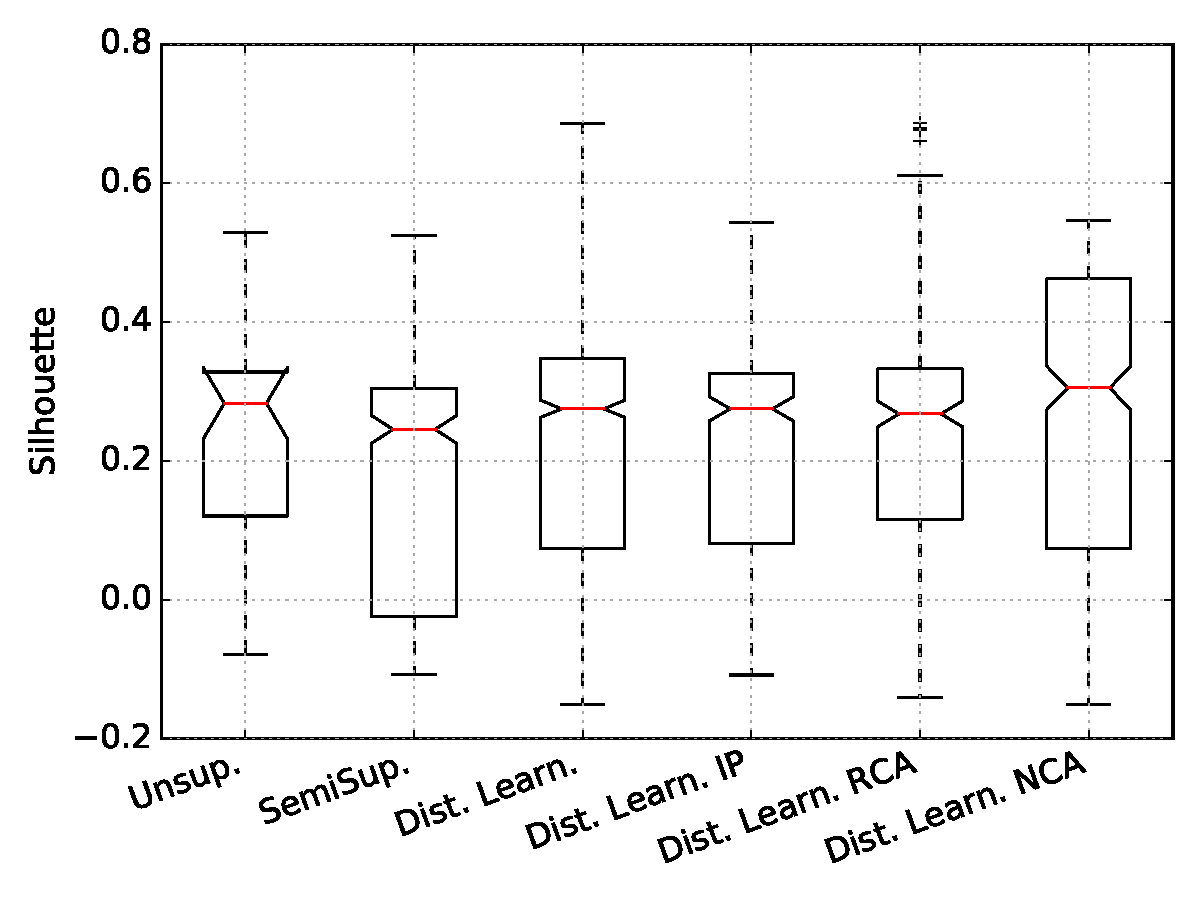
\includegraphics[width=0.75\columnwidth]{img/ANEW/Silhouette2.pdf}
	\caption{Boxplot of the Silhouette indices for the different scenarios}
	\label{fig:ANEWsilhouette}
\end{figure}	


\subsection{Objective metrics} \label{sec:ANEW:obj_results}
The Silhouette index is an objective quality metric that defines how much the clusters are compact and well separated. In order to do so, it defines for each sample $s$ a variable $a$ as the mean distance to all the samples in the same cluster and a variable $b$ as the mean distance to all the samples in the next nearest cluster. In order for a clustering to be well separated, $a$ should be small and $b$ should be high. The Silhouette index is hence computed as \cite{scikit-learn}:
\begin{equation}
\text{Silhouette}=\frac{1}{|\mathcal{D}|} \sum_{s \in \mathcal{D}} \frac{b-a}{\text{max}(a,b)}\in [-1,1],
\end{equation}
where $\mathcal{D}$ is the generic dataset of samples. 

High (positive) values of Silhouette indicate dense well-separated clusters, values around $0$ indicate overlapping clusters and low (or negative) values indicate incorrect clusters. 

In Figure \ref{fig:ANEWsilhouette} we show the boxplots of Silhouette metric for the different scenarios, while in Table \ref{tab:ANEWsilhouette} we show the configurations that generate the best results for each scenario. 

It is clear that the application of Distance Learning techniques outperforms unsupervised and semi-supervised techniques, even with different configurations of kernels, algorithms and constraints. In particular, the best performance is obtained with the Agglomerative Hierarchical Clustering over the third degree polynomial expansion of the VAD dataset, with a translation learned using the RCA technique constrained by the data collected from the Human Clustering. 

From the boxplot we can see that the RCA distance learning presents some extremely high values of Silhouette, which are considered outliers. Nevertheless, even without the supposed-outlier configurations, the RCA technique achieves the highest results for the Silhouette index. 

We can also notice that the semi-supervised scenario performs on average worse than the unsupervised scenario. This is because the Silhouette index evaluates the resulting clusters with respect of the position of the input data, that is not moved from the original position. The estimated clusters are therefore more noisy, which confirms the advantage of distance learning techniques to transform the space.


\begin{figure}[tbp]
	\centering %\includegraphics[width=0.75\columnwidth]{img/ANEW/ILMVscore.pdf}
 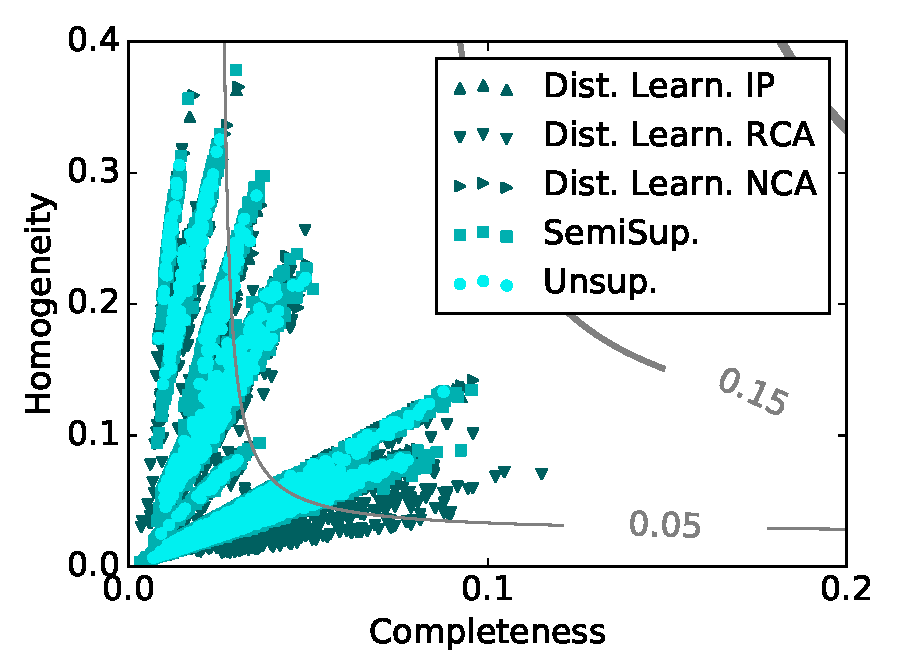
\includegraphics[width=.75\columnwidth]{img/ANEW/ILMVscore_square.pdf}
	\caption{Completeness and Homogeneity results for the comparison of clusters with those obtained from the ILM10K dataset. Gray contour lines indicate the V-score}
	\label{fig:ANEWILM10K}
\end{figure}


\subsection{Subjective metrics - Comparison with Clustering of ILM10K}
\label{sec:ANEW:subILM10K_results}
We compare the clusters obtained with the different approaches with the clusters obtained from ILM10K data. In this case, we have a set of predicted clusters and a set of ground truth clusters, and we want to estimate how much the former resembles the latter.  

We consider the homogeneity and completeness metrics \cite{rosenberg2007v}. The former evaluates whether each estimated cluster contains only members of a group in the ground truth, while the latter estimates whether the samples of a given group belongs to the same estimated cluster. We also consider the V-measure, i.e., the harmonic mean of homogeneity and completeness. 

To avoid overfitting issues, we evaluate only the configurations that are not trained with the constraints generated from the ILM10K dataset. 


We show the distribution of results for the different scenarios in Figure \ref{fig:ANEWILM10K}, where each point is a different configuration. We can visually estimate there are some stripes in the distribution of results, which are probably caused by the different sets of ground truth generated by the different clustering techniques and datasets from the ILM10K dataset. 
We notice the results are fairly low, showing that the organization given by the expanded and possibly learned ANEW dataset is very different from that obtained from editorial tags on a real music annotation application. This confirms the low correlation shown in Figure \ref{fig:ANEWdistData} and the necessity to find a space for the ANEW dataset which is more useful for MIR applications. However, it is clear that our approach can only slightly improve the task. 


\begin{table}[tbp]
    \small
\begin{center}
  \bgroup
  \def\arraystretch{1.5}
\begin{tabular}{ ||l  |l| l |l  |c|c|c ||}
\hline
\hline
Scenario 		& Features 		&  Alg. 	& Constr.  	& Compl. 	& Hom. 	& V-score \\
\hline
\hline
Unsup. 	& VA, poly 3 degree & SC &  &  0.0877 & 0.1334 & 0.1058 \\
\hline
Semi-Sup. & VAD poly 2 degree & AHC 		& $\mathbf{{M}}_{HD}$   & 0.0955 & 0.1347 & 0.1118 \\
\hline
IP Dist. & VA 			& SC 		& $\mathbf{{M}}_{HD}$   	& 0.0929 & 0.1371 & 0.1107 \\
\hline
RCA Dist. & VAD & kmeans & $\mathbf{{M}}_{HD}$ & 0.0869 & 0.1290 & {\color[HTML]{8E0000} \textit{0.1038}} \\
\hline
NCA Dist.& VA, poly 2 degree & AHC & $\mathbf{{M}}_{HD}$   & 0.0959 & 0.1421 & {\color[HTML]{326B00} \textbf{0.1145}}  \\
\hline
\hline
\end{tabular}
\egroup
\end{center}
\caption{Best results of the Homogeneity, Separation and V-measure metrics for the comparison with the clusters generated by the AHC from the normalized ILM10K dataset ($T=240$, $k=100$)}
\label{tab:ANEWv_score}
\end{table}

In Table \ref{tab:ANEWv_score} we list the configurations that lead to the best performance. Such configuration are able to achieve a V-Score between $0.1058$ and $0.1145$, which is quite low. From the range of the best results in the Completeness and Homogeneity values, we can infer that the best results are all generated from the same configuration of the ILM10K ground truth, i.e., the one composed by the Agglomerative Hierachical Clustering on the normalized dataset with 240 terms and $k=100$. This configuration is the most informative and reliable one, since it has few widely-used tags and the highest number of components, i.e., the richest approximation of the original matrix.  

Moreover, we can also see that all the highest results have been achieved by using the constraints from Human Distance. We believe that the reason of this is the medium-high correlation between the Human Distance annotation and the Normalized ILM10K dataset, as shown in Figure \ref{fig:ANEWdistData}.

The best results is reached using NCA technique with a AHC over the polynomial-expanded VA dataset. We can see that the dataset and the kernel is the same that obtained the second highest result for the Silhouette metrics in Table \ref{tab:ANEWsilhouette} for the NCA technique. Moreover, the AHC is also used for the two highest results in this case, the NCA distance learning technique and the Semi-Supervised clustering.

However, since all the results are rather low, we cannot draw meaningful conclusions from this evaluation.

\subsection{Subjective metrics - Comparison with Human Annotations}
\label{sec:ANEW:subHC_results}
We finally compare the obtained clusters with those collected from human clustering annotations (HC). For this case, we will use traditional Precision, Recall and F-Measure metrics, which focus more on the the correctly grouped terms rather than the correctly non-grouped ones, since the former are more specific and relevant.

We define the matrices $\mathbf{Y}\in \mathbb{R}^{T \times T}$ of HC annotation and $\hat{\mathbf{Y}}$ the estimated annotations, with $\mathbf{Y}(i,j)=1$ if the $i$-th and $j$-th samples are in the same cluster, we define the sets $TP$, $FP$ and $FN$ as:
\begin{equation}
TP=\{(i,j) : \mathbf{Y}(i,j)=\hat{\mathbf{Y}}(i,j)=1 \};
\end{equation}
\begin{equation}
FP=\{(i,j) : \mathbf{Y}(i,j)\neq 1=\hat{\mathbf{Y}}(i,j) \};
\end{equation}
\begin{equation}
FN=\{(i,j) : \mathbf{Y}(i,j)=1 \neq \hat{\mathbf{Y}}(i,j) \}; 
\end{equation}
with $i,j=1,...,T$ and  $i<j$ to avoid duplicate pairs of samples such as $(i,j)$ and $(j,i)$.

The Precision, Recall and F-Measure are defined as in previous Chapters as  $P= |TP|/(|TP|+|FP|) $, $R=|TP|/(|TP|+|FN|) $ and $F=2*P*R/(P+R)$ \cite{Manning2008}. 

To avoid overfitting, we evaluate only configurations that are not trained with the constraints generated from the human annotations on clustering.

\begin{figure}[tbp]
	\centering 
     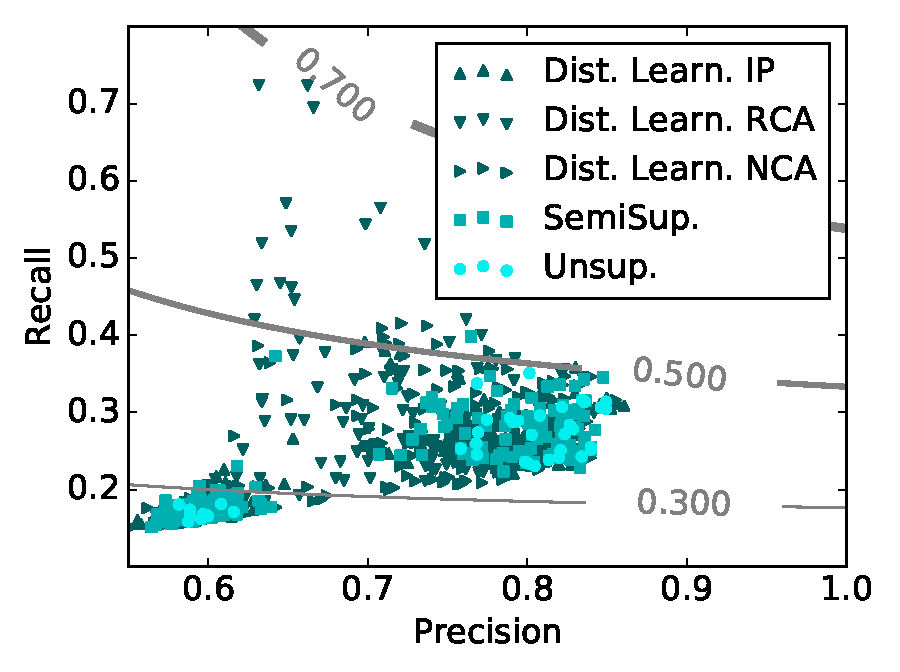
\includegraphics[width=.75\columnwidth]{img/ANEW/F_measure_square.pdf}
  %  \includegraphics[width=0.7\columnwidth,height=5cm]{img/ANEW/F_measure.pdf}    
	\caption{Precision and Recall results for the comparison of clusters with those obtained from human annotation. Gray contour lines indicate the F-measure.}
	\label{fig:ANEWF_measure}
\end{figure}	

In Figure \ref{fig:ANEWF_measure} we show the distribution of results for the different scenarios and configurations. In general, Precision is higher than Recall, showing that the estimated clustering is not capable of retrieving all the corrected groups, while it is effective of correctly estimating the clusters. The F-measures are mostly distributed between 0.3 and 0.5, which is an average result. In particular, we can notice two notable trends, one around $P=0.6$ and one around $P=0.8$.
However, we can clearly see that some configuration from RCA Distance Learning are able to improve the average Recall and achieve highest values of F-measure.  The F-measure is achieved by losing some effectiveness in the Precision, leading to a rather balanced performance between $P$ and $R$. We can see that at least $9$ RCA configurations obtained higher results than any other configurations, and only one Semi-Supervised technique achieves $F>.5$. This consideration clearly shows that the distance learning techniques are more effective to embed the information from constraints to better organize the terms with respect to the music context. 

\begin{table}[thb]
\begin{center}
  \bgroup
  \def\arraystretch{1.5}
\begin{tabular}{ ||l |l| l |p{.15\textwidth} |c  |c|c||}
\hline
\hline
Scenario 		& Features 		&  Algorithm 	& Constraints 		& P 	& R 	& F \\
\hline
\hline
Unsup. 	& VAD, RBF & kmeans 		& 				 &  0.8012 & 0.3512 & {\color[HTML]{8E0000} \textit{0.4883}} \\
\hline
Semi-Sup. & VAD, RBF & AHC 		& $\mathbf{{M}}_{HD}$   	& 0.7646 & 0.3986 & 0.5240 \\
\hline
IP Dist. & VAD, RBF & AHC 		& $\mathbf{\hat{M}}_{ILM10K}$, $T=240$,$\quad \;$ $k=100$ & 0.6979 & 0.3915 & 05016 \\
\hline
RCA Dist. & VA, poly 3 degree & AHC & $\mathbf{\hat{M}}_{ILM10K}$, $T=240$,$\quad \;$ $k=50$ & 0.6622 & 0.7241 & {\color[HTML]{326B00}  \textbf{0.6918}} \\
\hline
NCA Dist.& VAD, RBF & kmeans & $\mathbf{\hat{M}}_{ILM10K}$, $T=240$,$\quad \;$ $k=10$ & 0.7971 & 0.4124 & 0.5289  \\
\hline
\hline
\end{tabular}\quad
\egroup
\end{center}
\caption{Best results for the Precision, Recall and F-measure metric for the comparison with the human annotated clusters }
\label{tab:ANEWf_measure}
\end{table}

In Table \ref{tab:ANEWf_measure} we list the best configurations for each scenarios. The RCA Distance Learning technique clearly outperforms the other approaches and matches very closely the human annotations, i.e., the human organization of the emotional-related descriptors in the signal domain. We can notice that once again, the best results are obtained by using the AHC over some polynomial expansion of the dataset. Moreover, all the distance learning techniques take advantage of the constraints generated from the most informative set of annotations, i.e., the normalized ILM10K dataset with fewer terms. In this scenario, however, lower components are required to achieve higher results: the RCA distance learning achieves its best results with $k=50$ components and the NCA distance learning with just $k=10$ components.

\section{Final considerations}\label{sec:ANEW:conclusions}
In this Chapter we introduced a novel approach consisting of kernel expansion, constraint building from task specific human annotation and finally distance learning to transform the ANEW dataset and obtain a distribution of terms that provides better conceptual organization with respect to the conventional VA or VAD spaces.

We validate our approach by evaluating its ability to conceptually organize the terms by performing some clustering techniques on the expanded and learned space, using subjective and objective metrics. Average and maximum results prove that distance learning techniques are effective in the improvement of the organization of concepts of the ANEW dataset. In particular, agglomerative hierarchical clustering of a RCA-learned space based on the polynomial expansion of VA/VAD space outperforms the other configurations. 

This study investigates a possible formalization of the semantic codomain as a dimensional semantic model for emotional-related descriptors. While the VA model and the ANEW space have been used in the MIR community for several years, this study proposed an useful approach to improve its ability of describing and possibly retrieving music content.
